\documentclass[12pt]{article}
\usepackage[left=2cm,right=2cm,top=2cm,bottom=2cm]{geometry}
\usepackage{wrapfig}
\usepackage{booktabs}
\usepackage{graphicx}
\usepackage{amsmath}
\usepackage{siunitx} % Required for alignment
\usepackage{subfigure}
\usepackage{multirow}
\usepackage{rotating}
\usepackage[T2A]{fontenc}
\usepackage[english, russian]{babel}
\usepackage{caption}
\usepackage{hyperref}
\usepackage{float}

\hypersetup{
    colorlinks=true,
    linkcolor=red,
    urlcolor=magenta,
    }
\graphicspath{{pictures/}}


\title{\begin{center}Лабораторная работа №2.2.1\end{center} Исследование взаимной
диффузии газов} \author{Балдин Виктор
Б01-303} \date{\today}

\begin{document}
\maketitle

\textbf{Цель работы:} 1) регистрация зависимости концентрации гелия в воздухе
от времени при помощи датчиков теплопроводности при разных начальных давлениях
смеси газов;
2) определение коэффициента диффузии по данным измерений.

\textbf{В работе используются:} измерительная установка;
форвакуумный насос; баллон с газом (гелий); манометр; источник
питания; магазин сопротивлений; гальванометр; секундомер.

\section{Теоретическая часть}
\paragraph*{Взаимная диффузия газов}
Суммарное количество молекул в 2-х сосудах, разделенных перегородкой:
\begin{equation}
    N_1 + N_2 = V_1n_1 + V_2n_2 = const,
    \label{Neq}
\end{equation}
где $n_1$, $n_2$ -- концентрации.
Продифференцируем \ref{Neq} и в квазистационарном приближении запишем закон Фика:
\begin{equation}
    V_1dn_1 = -V_2dn_2 = Jdt = -DS\frac{n_1 - n_2}{l}dt,
    \label{fick}
\end{equation}
где $l$ -- длина трубки, $D$ -- коэффициент диффузии, $S$ -- площадь сечения.
Из системы \ref{fick}:
\begin{equation}
    \frac{dn_1}{dt} - \frac{dn_2}{dt} = -\frac{n_1 - n_2}{l}DS\left(\frac{1}{V_1}
        + \frac{1}{V_2}\right)
    \label{diffeq}
\end{equation}
Введя новую переменную $\Delta n = n_1 - n_2$ и проинтегрировав \ref{diffeq}, получим:
\begin{equation}
    \Delta n = \Delta n_0 e^{-t/\tau}
\end{equation}
Из начальных условий:
\begin{equation}
    \tau = \frac{V_1V_2}{V_1 + V_2}\frac{l}{SD},
\end{equation}
или
\begin{equation}
    D = \frac{V_1V_2}{V_1 + V_2}\frac{l}{S\tau}
    \label{diff_coeff}
\end{equation}

C другой стороны, считая плотностью гелия много меньше плотности воздуха,
можно утверждать, что
\begin{equation}
    D = \frac{1}{3}\lambda \left<v\right>,
    \label{diff}
\end{equation}
где $\lambda = \frac{1}{n\sigma}$ -- длина свободного пробега частиц, $\left<v\right> =
\sqrt{\frac{8RT}{\pi \mu}}$ -- средняя скорость теплового движения.

\paragraph*{Экспериментальная установка}
Для измерения $\Delta n$ применяется мостовая схема с термопарой (рис. \ref{schem}).
\begin{figure}
    \centering
    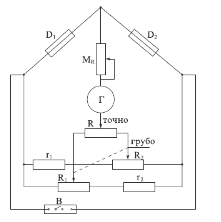
\includegraphics{stand.png}
    \caption{Мостовая схема с термопарой}
    \label{schem}
\end{figure}

Показания термопары пропорциональны $\Delta n$, а значит подчиняются закону
\begin{equation}
    \ln U = \ln U_0 - \frac{t}{\tau}
\end{equation}

\section{Ход работы}
\begin{enumerate}
    \item Откачаем воздух из установки, запустим гелий до рабочего давления.
    \item Сбалансируем мост.
    \item Откроем кран К3.
    \item Начнем измерения процесса диффузии.
    \item Повторим действия пп. 1-4 для 4-х значений рабочего давления.
    \item Соберем данные при помощи компьютеризованной установки при разных
    значениях рабочего давления.
    \item Получим графики зависимости $U(t)$ (рис. \ref{raw}) и $\ln U(t)$ (рис. \ref{lin}).
    Погрешность измерения времени и напряжения считаем пренебрежимо малой по сравнению
    с погрешностью измерения параметров установки.

    \begin{figure}[h!]
        \centering
        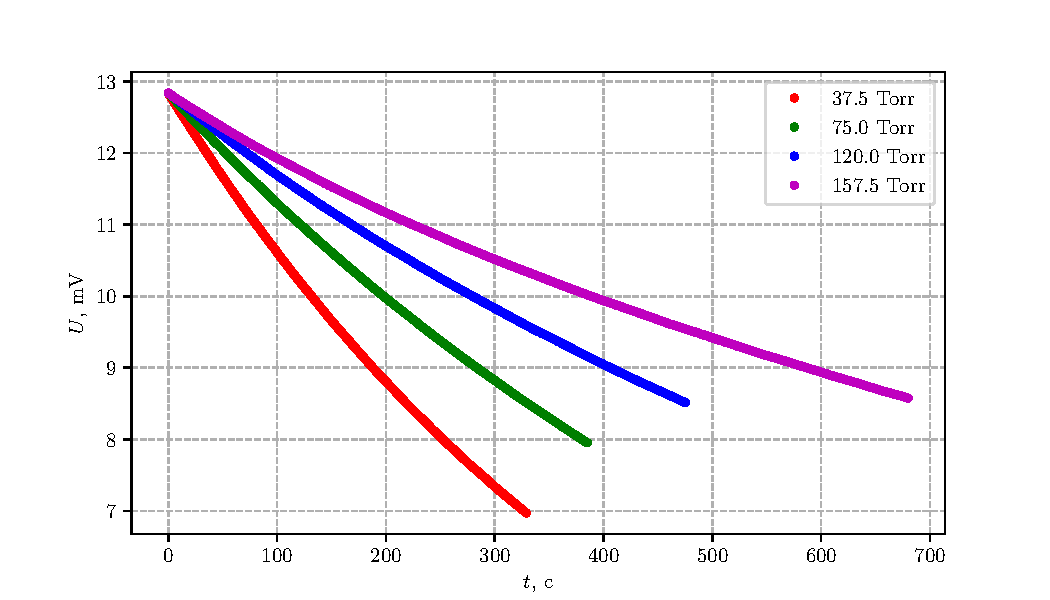
\includegraphics{raw.pdf}
        \caption{График $U(t)$}
        \label{raw}
    \end{figure}

    \begin{figure}[h!]
        \centering
        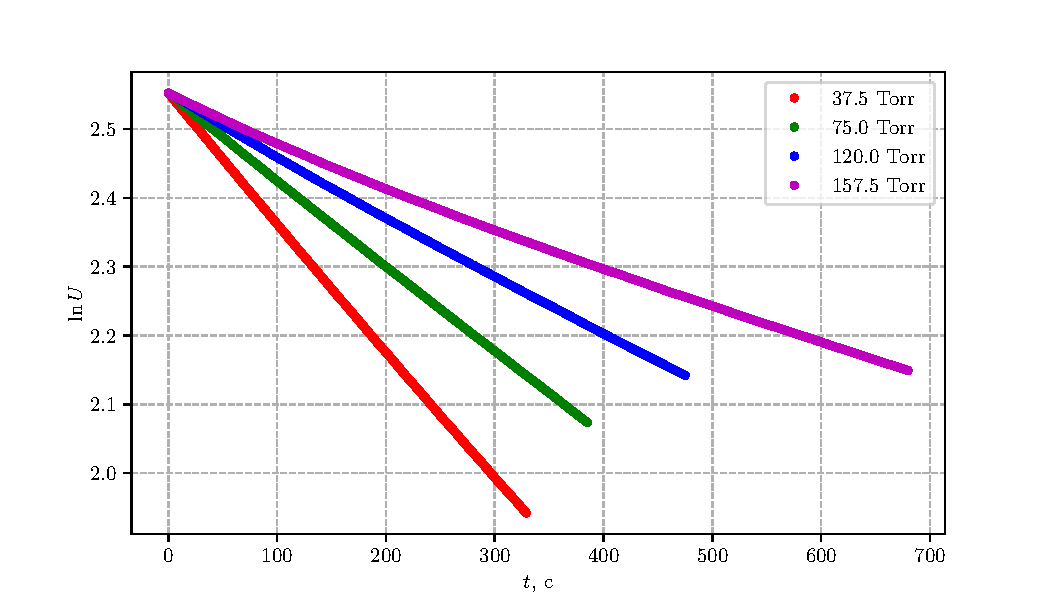
\includegraphics{lin.pdf}
        \caption{Линеаризованный график $\ln U(t)$}
        \label{lin}
    \end{figure}

    \item Полученные по формуле \ref{diff_coeff} коэффициенты диффузии при разных
    данных давлениях $D(P)$ представлены в таблице \ref{DP}. Погрешность $D$ оценим по следующей
    формуле:
    $$
    \varepsilon_D = \sqrt{\varepsilon_{V_1}^2 + \varepsilon_{V_2}^2 + \varepsilon_{l/S}^2
    + \varepsilon_{1/\tau}^2}
    $$
    Параметры установки:
    \begin{align*}
        V_1 & = (800\pm 5)\ \text{см}^3,\\
        V_2 & = (800\pm 5)\ \text{см}^3,\\
        \frac{l}{S} & = (15.0 \pm 0.1)\ \text{см}^{-1}.
    \end{align*}

    \begin{table}[h!]
        \centering
        \begin{tabular}{|r|r|r|r|r|r|r|}
        \toprule
         $P$, торр &  $-1/\tau$, $10^{-4}$ c$^{-1}$ &  $\Delta (-1/\tau)$, $10^{-4}$ c$^{-1}$ &  $\varepsilon_{-1/\tau}$, \% &  $D$, см$^2$/c &  $\Delta D$, см$^2$/c &  $\varepsilon_D$, \% \\
        \midrule
             37.50 &                      -18.58 &                                 0.01 &                        0.06 &                11.15 &                        0.12 &                 1.10 \\
             75.00 &                      -12.42 &                                 0.01 &                        0.04 &                 7.45 &                        0.08 &                 1.10 \\
            120.00 &                       -8.62 &                                 0.01 &                        0.11 &                 5.17 &                        0.06 &                 1.10 \\
            157.50 &                       -5.83 &                                 0.01 &                        0.21 &                 3.50 &                        0.04 &                 1.10 \\
        \bottomrule
        \end{tabular}
        \caption{Зависимость $D(P)$}
        \label{DP}
        \end{table}

    \item Построим график линеаризованной зависимости $D(1/P)$ (рис. \ref{D1P_graph}). Считаем, что
    прямая проходит через начало координат из теоретических соображений.
    \begin{figure}[h!]
        \centering
        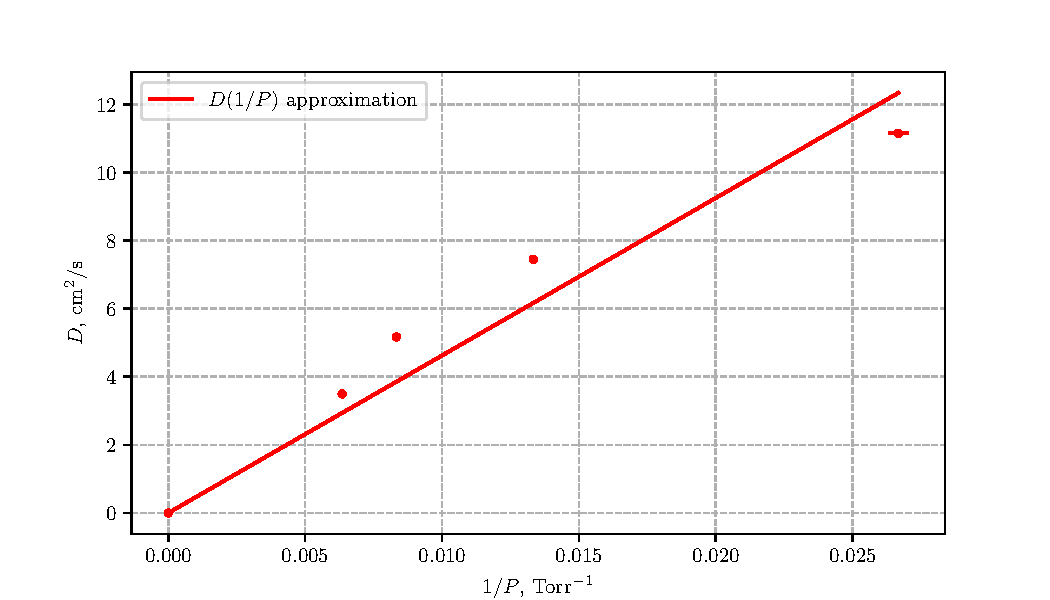
\includegraphics{diff.pdf}
        \caption{График $D(1/P)$}
        \label{D1P_graph}
    \end{figure}

    \item Из интерполяции зависимости найдем значение $D$ при атмосферном давлении:
    $$ D_0 = (0.61 \pm 0.06)\ \text{см}^2/\text{c},\ \varepsilon_{D_0} = 9 \% $$

    Отсюда по формуле \ref{diff} найдем остальные требуемые параметры:
    \begin{align*}
        \lambda & = (1.5 \pm 0.2) \cdot 10^{-7}\ \text{м},\ \varepsilon_{\lambda} = 10\%,\\
        \sigma & = (2.5 \pm 0.3) \cdot 10^{-19}\ \text{м}^2,\ \varepsilon_{\sigma} = 10\%.
    \end{align*}

\end{enumerate}
\section{Обсуждение результатов}
По графику \ref{D1P_graph} можно видеть, что линейное приближение $D(1/P)$ не слишком точно.
Возможной причиной является неточность приближения \ref{diff}. Поэтому и погрешность итогового
результата велика.

Однако, наши результаты находятся в некоторой близости к табличным:
\begin{align*}
    D_{\text{табл}} & = 0.62\ \text{см}^2/\text{c},\\
    \lambda_{\text{табл}} & = 1.75\cdot 10^{-7}\ \text{м},
\end{align*}
а значит качество модели можно считать в определенной степени удовлетворительным.

\end{document}
